% =============================================================================
%  B.Tech Project -- Mid-Semester Evaluation Report
%  Every result number in this file is a macro from generated/numbers.tex,
%  produced by report/build_tables.py from results/stage1/results_summary.json.
%  Do not type result numbers by hand; re-run build_tables.py instead.
% =============================================================================
\documentclass[11pt,a4paper]{article}
\usepackage[a4paper,margin=2.2cm]{geometry}
\usepackage[T1]{fontenc}
\usepackage{lmodern}
\usepackage{amsmath}
\usepackage{graphicx}
\usepackage{booktabs}
\usepackage{tabularx}
\usepackage{array}
\usepackage[font=small,labelfont=bf,skip=4pt]{caption}
\usepackage[compact]{titlesec}
\usepackage[hidelinks]{hyperref}
\usepackage{enumitem}
\usepackage{tikz}
\usetikzlibrary{positioning,arrows.meta,fit}

\setlist{nosep,leftmargin=1.4em}
\setlength{\parskip}{3pt}
\setlength{\parindent}{0pt}
\titlespacing*{\section}{0pt}{8pt}{3pt}
\titlespacing*{\subsection}{0pt}{6pt}{2pt}
\setlength{\textfloatsep}{8pt}
\setlength{\floatsep}{6pt}

% AUTO-GENERATED by report/build_tables.py from results_summary.json. Do not edit.
\newcommand{\accRepRest}{99.69\%}
\newcommand{\fRepRest}{99.69\%}
\newcommand{\accSegFiftyRest}{99.69\%}
\newcommand{\balSegFiftyRest}{99.69\%}
\newcommand{\voteSegFiftyRest}{14/14}
\newcommand{\accSubjFiftyRest}{62.73\%}
\newcommand{\balSubjFiftyRest}{62.73\%}
\newcommand{\voteSubjFiftyRest}{10/14}
\newcommand{\accSegZeroRest}{99.07\%}
\newcommand{\balSegZeroRest}{99.07\%}
\newcommand{\voteSegZeroRest}{14/14}
\newcommand{\accSubjZeroRest}{63.66\%}
\newcommand{\balSubjZeroRest}{63.66\%}
\newcommand{\voteSubjZeroRest}{9/14}
\newcommand{\accGlobalRest}{99.69\%}
\newcommand{\accRawSegRest}{100.00\%}
\newcommand{\accRawSubjRest}{66.15\%}
\newcommand{\voteRawSubjRest}{9/14}
\newcommand{\tiesRest}{0}
\newcommand{\silClassRest}{0.075}
\newcommand{\silSubjRest}{0.218}
\newcommand{\subjIDRest}{98.91\%}
\newcommand{\subjIDchanceRest}{7.14\%}
\newcommand{\nSegRest}{644}
\newcommand{\nSegCtlRest}{322}
\newcommand{\nSegDisRest}{322}
\newcommand{\nSubjRest}{14}
\newcommand{\nSubjCtlRest}{7}
\newcommand{\nSubjDisRest}{7}
\newcommand{\nSegZeroRest}{322}
\newcommand{\nSegPerSubjMinRest}{46}
\newcommand{\nSegPerSubjMaxRest}{46}
\newcommand{\nFeatRest}{126}
\newcommand{\nFoldsSubjRest}{14}
\newcommand{\nBelowHalfRest}{4}
\newcommand{\nZeroRest}{3}
\newcommand{\nPerfectRest}{4}
\newcommand{\accRepMusic}{96.43\%}
\newcommand{\fRepMusic}{96.43\%}
\newcommand{\accSegFiftyMusic}{96.43\%}
\newcommand{\balSegFiftyMusic}{96.43\%}
\newcommand{\voteSegFiftyMusic}{14/14}
\newcommand{\accSubjFiftyMusic}{43.01\%}
\newcommand{\balSubjFiftyMusic}{43.01\%}
\newcommand{\voteSubjFiftyMusic}{8/14}
\newcommand{\accSegZeroMusic}{94.41\%}
\newcommand{\balSegZeroMusic}{94.41\%}
\newcommand{\voteSegZeroMusic}{14/14}
\newcommand{\accSubjZeroMusic}{50.62\%}
\newcommand{\balSubjZeroMusic}{50.62\%}
\newcommand{\voteSubjZeroMusic}{8/14}
\newcommand{\accGlobalMusic}{94.10\%}
\newcommand{\accRawSegMusic}{99.22\%}
\newcommand{\accRawSubjMusic}{67.55\%}
\newcommand{\voteRawSubjMusic}{8/14}
\newcommand{\tiesMusic}{0}
\newcommand{\silClassMusic}{0.066}
\newcommand{\silSubjMusic}{0.193}
\newcommand{\subjIDMusic}{99.07\%}
\newcommand{\subjIDchanceMusic}{7.14\%}
\newcommand{\nSegMusic}{644}
\newcommand{\nSegCtlMusic}{322}
\newcommand{\nSegDisMusic}{322}
\newcommand{\nSubjMusic}{14}
\newcommand{\nSubjCtlMusic}{7}
\newcommand{\nSubjDisMusic}{7}
\newcommand{\nSegZeroMusic}{322}
\newcommand{\nSegPerSubjMinMusic}{46}
\newcommand{\nSegPerSubjMaxMusic}{46}
\newcommand{\nFeatMusic}{126}
\newcommand{\nFoldsSubjMusic}{14}
\newcommand{\nBelowHalfMusic}{6}
\newcommand{\nZeroMusic}{2}
\newcommand{\nPerfectMusic}{0}
\newcommand{\accRepRestMusic}{99.77\%}
\newcommand{\fRepRestMusic}{99.77\%}
\newcommand{\accSegFiftyRestMusic}{99.77\%}
\newcommand{\balSegFiftyRestMusic}{99.77\%}
\newcommand{\voteSegFiftyRestMusic}{14/14}
\newcommand{\accSubjFiftyRestMusic}{62.34\%}
\newcommand{\balSubjFiftyRestMusic}{62.34\%}
\newcommand{\voteSubjFiftyRestMusic}{9/14}
\newcommand{\accSegZeroRestMusic}{99.22\%}
\newcommand{\balSegZeroRestMusic}{99.22\%}
\newcommand{\voteSegZeroRestMusic}{14/14}
\newcommand{\accSubjZeroRestMusic}{63.51\%}
\newcommand{\balSubjZeroRestMusic}{63.51\%}
\newcommand{\voteSubjZeroRestMusic}{10/14}
\newcommand{\accGlobalRestMusic}{99.77\%}
\newcommand{\accRawSegRestMusic}{100.00\%}
\newcommand{\accRawSubjRestMusic}{67.62\%}
\newcommand{\voteRawSubjRestMusic}{9/14}
\newcommand{\tiesRestMusic}{0}
\newcommand{\silClassRestMusic}{0.067}
\newcommand{\silSubjRestMusic}{0.173}
\newcommand{\subjIDRestMusic}{99.30\%}
\newcommand{\subjIDchanceRestMusic}{7.14\%}
\newcommand{\nSegRestMusic}{1288}
\newcommand{\nSegCtlRestMusic}{644}
\newcommand{\nSegDisRestMusic}{644}
\newcommand{\nSubjRestMusic}{14}
\newcommand{\nSubjCtlRestMusic}{7}
\newcommand{\nSubjDisRestMusic}{7}
\newcommand{\nSegZeroRestMusic}{644}
\newcommand{\nSegPerSubjMinRestMusic}{92}
\newcommand{\nSegPerSubjMaxRestMusic}{92}
\newcommand{\nFeatRestMusic}{126}
\newcommand{\nFoldsSubjRestMusic}{14}
\newcommand{\nBelowHalfRestMusic}{5}
\newcommand{\nZeroRestMusic}{0}
\newcommand{\nPerfectRestMusic}{1}
\newcommand{\accRepAdhd}{85.81\%}
\newcommand{\fRepAdhd}{85.79\%}
\newcommand{\accSegFiftyAdhd}{85.81\%}
\newcommand{\balSegFiftyAdhd}{85.49\%}
\newcommand{\voteSegFiftyAdhd}{121/121}
\newcommand{\accSubjFiftyAdhd}{57.54\%}
\newcommand{\balSubjFiftyAdhd}{57.09\%}
\newcommand{\voteSubjFiftyAdhd}{74/121}
\newcommand{\accSegZeroAdhd}{74.86\%}
\newcommand{\balSegZeroAdhd}{74.33\%}
\newcommand{\voteSegZeroAdhd}{109/121}
\newcommand{\accSubjZeroAdhd}{58.04\%}
\newcommand{\balSubjZeroAdhd}{57.53\%}
\newcommand{\voteSubjZeroAdhd}{79/121}
\newcommand{\accRawSegAdhd}{87.49\%}
\newcommand{\accRawSubjAdhd}{57.23\%}
\newcommand{\voteRawSubjAdhd}{69/121}
\newcommand{\tiesAdhd}{3}
\newcommand{\silClassAdhd}{0.026}
\newcommand{\silSubjAdhd}{-0.150}
\newcommand{\subjIDAdhd}{65.39\%}
\newcommand{\subjIDchanceAdhd}{0.83\%}
\newcommand{\nSegAdhd}{6588}
\newcommand{\nSegCtlAdhd}{2908}
\newcommand{\nSegDisAdhd}{3680}
\newcommand{\nSubjAdhd}{121}
\newcommand{\nSubjCtlAdhd}{60}
\newcommand{\nSubjDisAdhd}{61}
\newcommand{\nSegZeroAdhd}{3322}
\newcommand{\nSegPerSubjMinAdhd}{23}
\newcommand{\nSegPerSubjMaxAdhd}{134}
\newcommand{\nFeatAdhd}{171}
\newcommand{\nFoldsSubjAdhd}{10}
\newcommand{\nBelowHalfAdhd}{46}
\newcommand{\nZeroAdhd}{0}
\newcommand{\nPerfectAdhd}{0}
\newcommand{\precRepAdhd}{85.79\%}
\newcommand{\recRepAdhd}{85.81\%}
\newcommand{\mccRepAdhd}{0.712}
\newcommand{\kappaRepAdhd}{0.712}
\newcommand{\modeMeanDsOne}{10.78}
\newcommand{\modeSdDsOne}{3.29}
\newcommand{\modeMinDsOne}{4}
\newcommand{\modeMaxDsOne}{20}
\newcommand{\modeCapDsOne}{5.7\%}
\newcommand{\modeCtlDsOne}{10.19}
\newcommand{\modeDisDsOne}{11.37}
\newcommand{\modeMeanDsTwo}{4.55}
\newcommand{\modeSdDsTwo}{1.93}
\newcommand{\modeMinDsTwo}{1}
\newcommand{\modeMaxDsTwo}{19}
\newcommand{\modeCapDsTwo}{0.0\%}
\newcommand{\modeCtlDsTwo}{4.31}
\newcommand{\modeDisDsTwo}{4.74}


\begin{document}

% ------------------------------------------------------------------ title page
% Layout follows the IIT Indore BTP template (BTP_Latex_template.zip).
\begin{titlepage}
\begin{center}
\vspace*{1.2cm}
{\Large \bf EEG-based Multiple Neurodevelopmental\\[2pt] Disorders Detection} \\
\vspace{22pt}
{\large \bf B.Tech.\ Project -- Mid-Semester Evaluation Report}\\
\vspace{30pt}
\emph{Submitted in partial fulfillment of the requirements \\ of the degree of}\\[4pt]
{\large \bf Bachelor of Technology} \\
{\large in}\\
{\large \bf [Discipline]}\\
\vspace{30pt}
By \\
\vspace{10pt}
{\large \bf [Student Name]} \\
(Roll No: [roll no.])\\
\vspace{15pt}
Under the guidance of\\
{\large \bf [Prof.\ Supervisor Name]}\\
{[Designation, Department]}\\
\vspace{6pt}
Co-supervisor: [name or ``None'']\\
\vspace{30pt}

\includegraphics[width=5cm]{figures/IITI.png}\\
\vspace{20pt}
{\Large \bf [Department Name] \\
 Indian Institute of Technology Indore \\
 September 2026\\}
\end{center}
\end{titlepage}

\setcounter{page}{1}

% =================================================================== 1
\section{Introduction, Motivation and Theme}

Neurodevelopmental disorders are conditions that emerge during childhood
development and affect cognition, communication, attention or behaviour.
This project concerns two of them. Intellectual and developmental
disorder (IDD) is marked by limitations in reasoning and in adaptive
functioning across everyday settings, and attention-deficit/hyperactivity
disorder (ADHD) by sustained inattention, hyperactivity or impulsivity that
interferes with daily life. In both cases, support
started early in childhood tends to be more useful than support started late,
so tools that help flag children for specialist assessment have practical
value. Current diagnosis rests on clinical interviews and behavioural rating
scales, which require trained staff and depend on observer judgement.

Electroencephalography (EEG) is an attractive complementary signal for this
purpose. It is non-invasive, inexpensive relative to other neuroimaging, well
tolerated by children, and resolves brain activity on a millisecond scale.
Portable headsets make recording possible outside hospitals; one of the two
datasets used here was collected with a consumer-grade 14-channel device
\cite{sareen2020data}. EEG is, however, non-stationary, noisy and highly
individual, which has made signal decomposition methods and machine learning a
common route from raw recordings to a diagnostic decision.

Published EEG classifiers for IDD and ADHD frequently report accuracies close
to perfect on cohorts of a few dozen children. How such figures are obtained
matters as much as the figures themselves. A long recording from each child is
usually cut into many short windows, and if windows from the same child are
allowed into both the training and the test partitions, a classifier can
succeed by recognising the child rather than the disorder. Choosing features
or hyperparameters on the full dataset before validation adds a similar
optimistic bias. A screening tool is always applied to children it
has never seen, so the estimate that matters clinically is the
subject-independent one.

The theme of this project is therefore twofold: to reproduce a recent unified
EEG pipeline for IDD and ADHD detection \cite{chandela2025}, and to examine,
with evaluation protocols that keep each child on one side of the split, what
that pipeline learns and how well it transfers to new children.

% =================================================================== 2
\section{Project Objective and Problem Statement}

Given multichannel EEG from children with IDD or ADHD and from typically
developing controls, the task is binary classification of each child's
diagnostic group. The objectives are:
\begin{enumerate}
  \item Reproduce the SMVMD-based pipeline of \cite{chandela2025} end to end
        on both public datasets, as open, re-runnable code.
  \item Evaluate the reproduced pipeline under subject-independent protocols
        (leave-one-subject-out and grouped cross-validation) and report
        child-level as well as segment-level accuracy.
  \item Identify which components and signal properties drive
        classification, separating disorder-related information from
        child-specific signatures and dataset confounds.
\end{enumerate}

% =================================================================== 3
\section{Brief Literature Survey}

\textbf{EEG-based IDD detection.} Most EEG work on IDD has used the public
dataset of Sareen et al.\ \cite{sareen2020data}, recorded at rest and during
music listening. The studies reviewed in \cite{chandela2025} range from wavelet
sub-band features with a quadratic discriminant classifier (Anwar, 2020) and
fine-grained spectral band power with a random forest (Breitenbach et al.,
2021), to Morlet scalograms classified by a 3-D convolutional network (Oda and
Norouzi, 2021) and a deep network operating on estimated cortical source
activity (Shah et al., 2023).

\textbf{EEG-based ADHD detection.} For ADHD, the same review
\cite{chandela2025} lists deep models such as EEGNet on event-related
recordings (Vahid et al., 2019) and convolutional networks applied to
connectivity matrices (Chen et al., 2019) or to EEG rendered as images
(Moghaddari et al., 2020). Several studies on the public ADHD recordings used
in this project \cite{motie2020} pair a signal decomposition with a learned
classifier: multivariate empirical mode decomposition with an artificial neural
network (Sharma and Singh, 2023), robust local mean decomposition combined with
VMD and a CNN (Esas and Latifo\u{g}lu, 2023), and multitaper spectra with MVMD
features and a CNN--LSTM (Kasim, 2023).

\textbf{Decomposition methods.} Decomposition splits an EEG channel into a
small number of oscillatory components that can be described separately.
Empirical mode decomposition (EMD) does this by iterative envelope sifting; it
adapts to the data but is prone to mode mixing. Variational mode decomposition
(VMD) instead solves an optimisation problem that finds a preset number of
band-limited modes around adaptively estimated centre frequencies, and its
multivariate form (MVMD) makes each mode share one centre frequency across all
channels. Successive VMD (SVMD) extracts modes one at a time until the residual
is exhausted, so their number need not be fixed in advance, and successive
multivariate VMD (SMVMD) combines both ideas for multichannel data. The
pipeline reproduced here uses SMVMD and therefore has to handle a different
number of modes in every window; formulations are given in \cite{chandela2025}
and the references therein.

\textbf{Evaluation design in EEG classification.} A recording of a few minutes
yields dozens of short, overlapping windows per child, and windows from one
child resemble each other far more than windows from different children. If
windows are assigned to folds at random, almost every test window has close
relatives from the same child in the training set, and the resulting accuracy
reflects recognition of known children rather than generalisation to new
ones. Selecting features or tuning hyperparameters on all windows before
cross-validation adds a further optimistic bias. The studies in
Table~\ref{tab:lit} use $k$-fold or hold-out validation, but whether their
splits separate children is not stated in the review of \cite{chandela2025};
Section~\ref{sec:new} measures the effect directly for the reproduced pipeline.

\begin{table}[t]
\centering\footnotesize
\caption{Representative EEG methods for IDD and ADHD detection, as reviewed
in \cite{chandela2025}. Validation is as reported there; whether the splits
separate children is not stated.}
\label{tab:lit}
\begin{tabularx}{\textwidth}{l l X l l}
\toprule
Work & Target, data & Representation & Classifier & Validation \\
\midrule
Anwar (2020) & IDD, \cite{sareen2020data} & Wavelet sub-band features & QDA & 7-fold CV \\
Breitenbach et al.\ (2021) & IDD, \cite{sareen2020data} & Fine-grained spectral band power & Random forest & 7-fold CV \\
Oda and Norouzi (2021) & IDD, \cite{sareen2020data} & Morlet scalograms & 3-D CNN & 71:29 hold-out \\
Shah et al.\ (2023) & IDD, \cite{sareen2020data} & Cortical source signals & ETSNet & 70:30, 7-fold CV \\
Chen et al.\ (2019) & ADHD, other cohort & Connectivity matrix & CNN & not reported \\
Moghaddari et al.\ (2020) & ADHD, other cohort & EEG rendered as images & CNN & not reported \\
Sharma and Singh (2023) & ADHD, \cite{motie2020} & Multivariate EMD, GA selection & ANN & not reported \\
Esas and Latifo\u{g}lu (2023) & ADHD, \cite{motie2020} & Robust local mean decomp.\ + VMD & CNN & not reported \\
Kasim (2023) & ADHD, \cite{motie2020} & Multitaper + MVMD features & CNN, Bi-LSTM & not reported \\
Chandela et al.\ \cite{chandela2025} & IDD + ADHD, both & SMVMD, energy-integrated features & KNN & 10-fold CV \\
\bottomrule
\end{tabularx}
\end{table}

% =================================================================== 4
\section{Work Done and Results}

\subsection{Pipeline as implemented}

Figure~\ref{fig:pipeline} shows the pipeline as implemented in Python for this
project. DS-1 \cite{sareen2020data} contains \nSubjDisRest{} children with IDD
and \nSubjCtlRest{} typically developing controls (TDC), each recorded with a
14-channel headset at rest and while listening to music. DS-2 \cite{motie2020}
contains \nSubjDisAdhd{} children with ADHD and \nSubjCtlAdhd{} normal controls
(NC), recorded with 19 electrodes during a visual attention task. DS-1 uses the
cleaned recordings distributed with the dataset; DS-2 is band-pass filtered,
notch filtered and wavelet denoised as described in \cite{chandela2025}. Both
are cut into 5\,s windows with 50\% overlap, which yields \nSegRest{} windows
per DS-1 condition, \nSegRestMusic{} for rest and music combined, and
\nSegAdhd{} for DS-2 (\nSegDisAdhd{} ADHD, \nSegCtlAdhd{} NC), the same counts
as stated in \cite{chandela2025}.

Each window is decomposed by SMVMD into $K$ multichannel modes, where $K$
varies from window to window. Nine descriptors are computed for every mode on
every channel (standard deviation, variance, RMS, interquartile range, absolute
sum of square roots, average power, maximum fractal length, information
potential and parametric-centred correntropy). To obtain a fixed-length vector
whatever the value of $K$, the features of channel $c$ are combined across
modes with energy weights \cite{chandela2025}:
\begin{equation}
  f_{c,m} \;=\; \frac{\sum_{k=1}^{K} f_{c,m,k}\, e_{c,k}}{\sum_{k=1}^{K} e_{c,k}},
  \qquad e_{c,k} = \sum_{t} u_{k,c}^2(t),
  \label{eq:energy}
\end{equation}
where $f_{c,m,k}$ is feature $m$ of mode $k$ on channel $c$ and $u_{k,c}$ is
that mode's waveform. This gives \nFeatRest{} features for DS-1 and \nFeatAdhd{} for DS-2. The
features are ranked by minimum-redundancy maximum-relevance (mRMR)
and classified with $k$-nearest neighbours using the
hyperparameters listed in Table~II of \cite{chandela2025}; the Bayesian search
that produced them was not re-run. In my implementation, standardisation,
mRMR and the classifier are fitted inside each training fold as a single
pipeline, which is stricter than fitting them once on all data.

\begin{figure}[t]
\centering
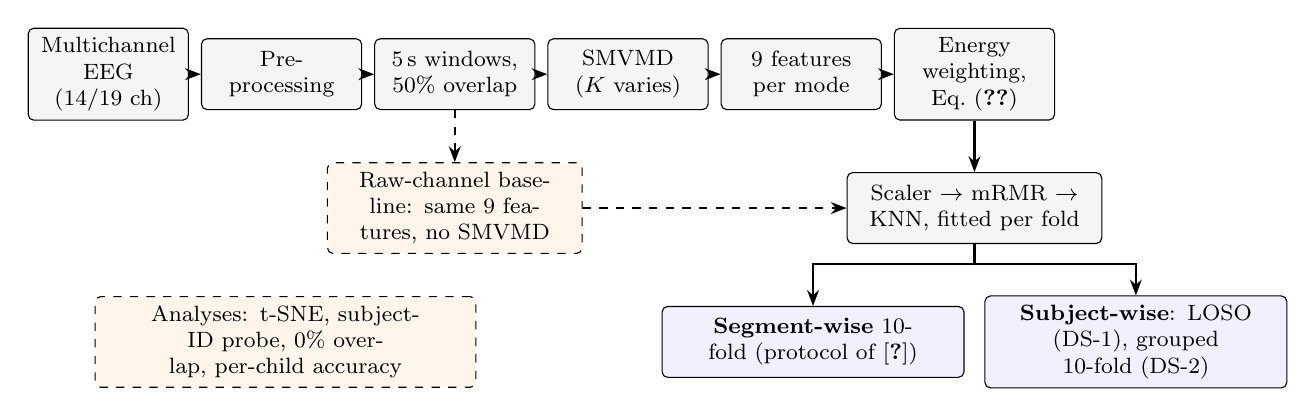
\begin{tikzpicture}[
  box/.style={draw, rounded corners=2pt, align=center, font=\footnotesize,
              minimum height=9mm, text width=18mm, fill=gray!8},
  ev/.style={box, text width=36mm, fill=blue!6},
  side/.style={box, fill=orange!8, dashed},
  arr/.style={-{Stealth[length=2mm]}, thick}]
% row 1: reproduced pipeline
\node[box] (eeg)   at (9.5mm,0)   {Multichannel EEG (14/19 ch)};
\node[box] (pre)   at (31.5mm,0)  {Pre-processing};
\node[box] (win)   at (53.5mm,0)  {5\,s windows, 50\% overlap};
\node[box] (smvmd) at (75.5mm,0)  {SMVMD ($K$ varies)};
\node[box] (feat)  at (97.5mm,0)  {9 features per mode};
\node[box] (int)   at (119.5mm,0) {Energy weighting, Eq.~(\ref{eq:energy})};
% row 2
\node[side, text width=30mm] (raw) at (53.5mm,-17mm) {Raw-channel baseline: same 9 features, no SMVMD};
\node[box, text width=30mm] (clf) at (119.5mm,-17mm) {Scaler $\rightarrow$ mRMR $\rightarrow$ KNN, fitted per fold};
% row 3: evaluation
\node[side, text width=46mm] (ana) at (32mm,-34mm) {Analyses: t-SNE, subject-ID probe, 0\% overlap, per-child accuracy};
\node[ev] (seg) at (99mm,-34mm) {\textbf{Segment-wise} 10-fold (protocol of \cite{chandela2025})};
\node[ev] (sub) at (140mm,-34mm) {\textbf{Subject-wise}: LOSO (DS-1), grouped 10-fold (DS-2)};
\draw[arr] (eeg) -- (pre); \draw[arr] (pre) -- (win); \draw[arr] (win) -- (smvmd);
\draw[arr] (smvmd) -- (feat); \draw[arr] (feat) -- (int); \draw[arr] (int) -- (clf);
\draw[arr, dashed] (win) -- (raw);
\draw[arr, dashed] (raw) -- (clf);
\draw[arr] (clf.south) -- ++(0,-2.5mm) -| (seg.north);
\draw[arr] (clf.south) -- ++(0,-2.5mm) -| (sub.north);
\end{tikzpicture}
\caption{Pipeline and evaluation design used in this project. Solid boxes
reproduce \cite{chandela2025}; blue boxes are the two evaluation protocols;
dashed boxes are the additional analyses of Section~\ref{sec:new}.}
\label{fig:pipeline}
\end{figure}

\subsection{Reproduction results}

Table~\ref{tab:repro} lists the reproduced results under the segment-wise
protocol of \cite{chandela2025}. The DS-1 settings reach between \accRepMusic{}
and \accRepRestMusic{}. On DS-2 the pipeline reaches \accRepAdhd{}, with an MCC
of \mccRepAdhd{} and Cohen's $\kappa$ of \kappaRepAdhd{}.

\begin{table}[t]
\centering\footnotesize
\caption{Reproduced results, segment-wise stratified 10-fold cross-validation.
Precision and recall are class-weighted averages.}
\label{tab:repro}
\begin{tabular}{lcccccl}
\toprule
Setting & Segments & Features & Accuracy & Precision & Recall & KNN (Table II of \cite{chandela2025})\\
\midrule
DS-1 Rest & 644 & 80 & 99.69\% & 99.69\% & 99.69\% & $k{=}2$, city-block, equal, std. \\
DS-1 Music & 644 & 47 & 96.43\% & 96.43\% & 96.43\% & $k{=}2$, city-block, sq.\ inverse \\
DS-1 Rest+Music & 1288 & 103 & 99.77\% & 99.77\% & 99.77\% & $k{=}1$, Euclidean, sq.\ inverse, std. \\
DS-2 & 6588 & 171 & 85.81\% & 85.79\% & 85.81\% & $k{=}2$, cosine, sq.\ inverse \\
\bottomrule
\end{tabular}

\end{table}

\subsection{Subject-independent evaluation and diagnostic analyses}
\label{sec:new}

\textbf{Segment-wise versus subject-wise.} Table~\ref{tab:protocols} evaluates
the identical pipeline under both protocols. The subject-wise protocol holds
out every window of a child together: leave-one-subject-out (LOSO, \nFoldsSubjRest{} folds)
for DS-1 and grouped 10-fold for DS-2. Each child is also assigned the majority
label of its held-out windows. Accuracy falls in every setting, for example
from \accSegFiftyRest{} to \accSubjFiftyRest{} for DS-1 rest and from
\accSegFiftyAdhd{} to \accSubjFiftyAdhd{} for DS-2, where \voteSubjFiftyAdhd{}
children are classified correctly.

\begin{table}[t]
\centering\footnotesize\setlength{\tabcolsep}{4pt}
\caption{Accuracy of the same pipeline under segment-wise (10-fold) and
subject-wise (LOSO for DS-1, grouped 10-fold for DS-2) cross-validation.
``Children'' counts correctly classified children by majority vote in the
subject-wise protocol. Balanced accuracy corrects for the class imbalance of
DS-2.}
\label{tab:protocols}
\begin{tabular}{l cccc cc cc}
\toprule
 & \multicolumn{4}{c}{SMVMD features, 50\% overlap} & \multicolumn{2}{c}{SMVMD, 0\% overlap} & \multicolumn{2}{c}{Raw channels, 50\%}\\
\cmidrule(lr){2-5}\cmidrule(lr){6-7}\cmidrule(lr){8-9}
Setting & Seg-wise & Subj-wise & Subj bal.\ acc. & Children & Seg-wise & Subj-wise & Seg-wise & Subj-wise\\
\midrule
DS-1 Rest & 99.69\% & 62.73\% & 62.73\% & 10/14 & 99.07\% & 63.66\% & 100.00\% & 66.15\% \\
DS-1 Music & 96.43\% & 43.01\% & 43.01\% & 8/14 & 94.41\% & 50.62\% & 99.22\% & 67.55\% \\
DS-1 Rest+Music & 99.77\% & 62.34\% & 62.34\% & 9/14 & 99.22\% & 63.51\% & 100.00\% & 67.62\% \\
DS-2 & 85.81\% & 57.54\% & 57.09\% & 74/121 & 74.86\% & 58.04\% & 87.49\% & 57.23\% \\
\bottomrule
\end{tabular}

\end{table}

\textbf{Window overlap (0\%).} The window (640 samples) is twice the step,
so the non-overlapping windows are exactly the even-numbered 50\%-overlap
windows. Since SMVMD and the features act on each window alone, the
0\%-overlap results reuse the cached features (\nSegZeroRest{} windows per
DS-1 condition, \nSegZeroAdhd{} for DS-2).

\textbf{Feature selection on all data.} Fitting the mRMR ranking once on every
window before cross-validation, as described in \cite{chandela2025}, gave
\accGlobalRest{} (rest), \accGlobalMusic{} (music) and \accGlobalRestMusic{}
(combined), equal to or below the fold-internal ranking.

\begin{figure}[t]
\centering
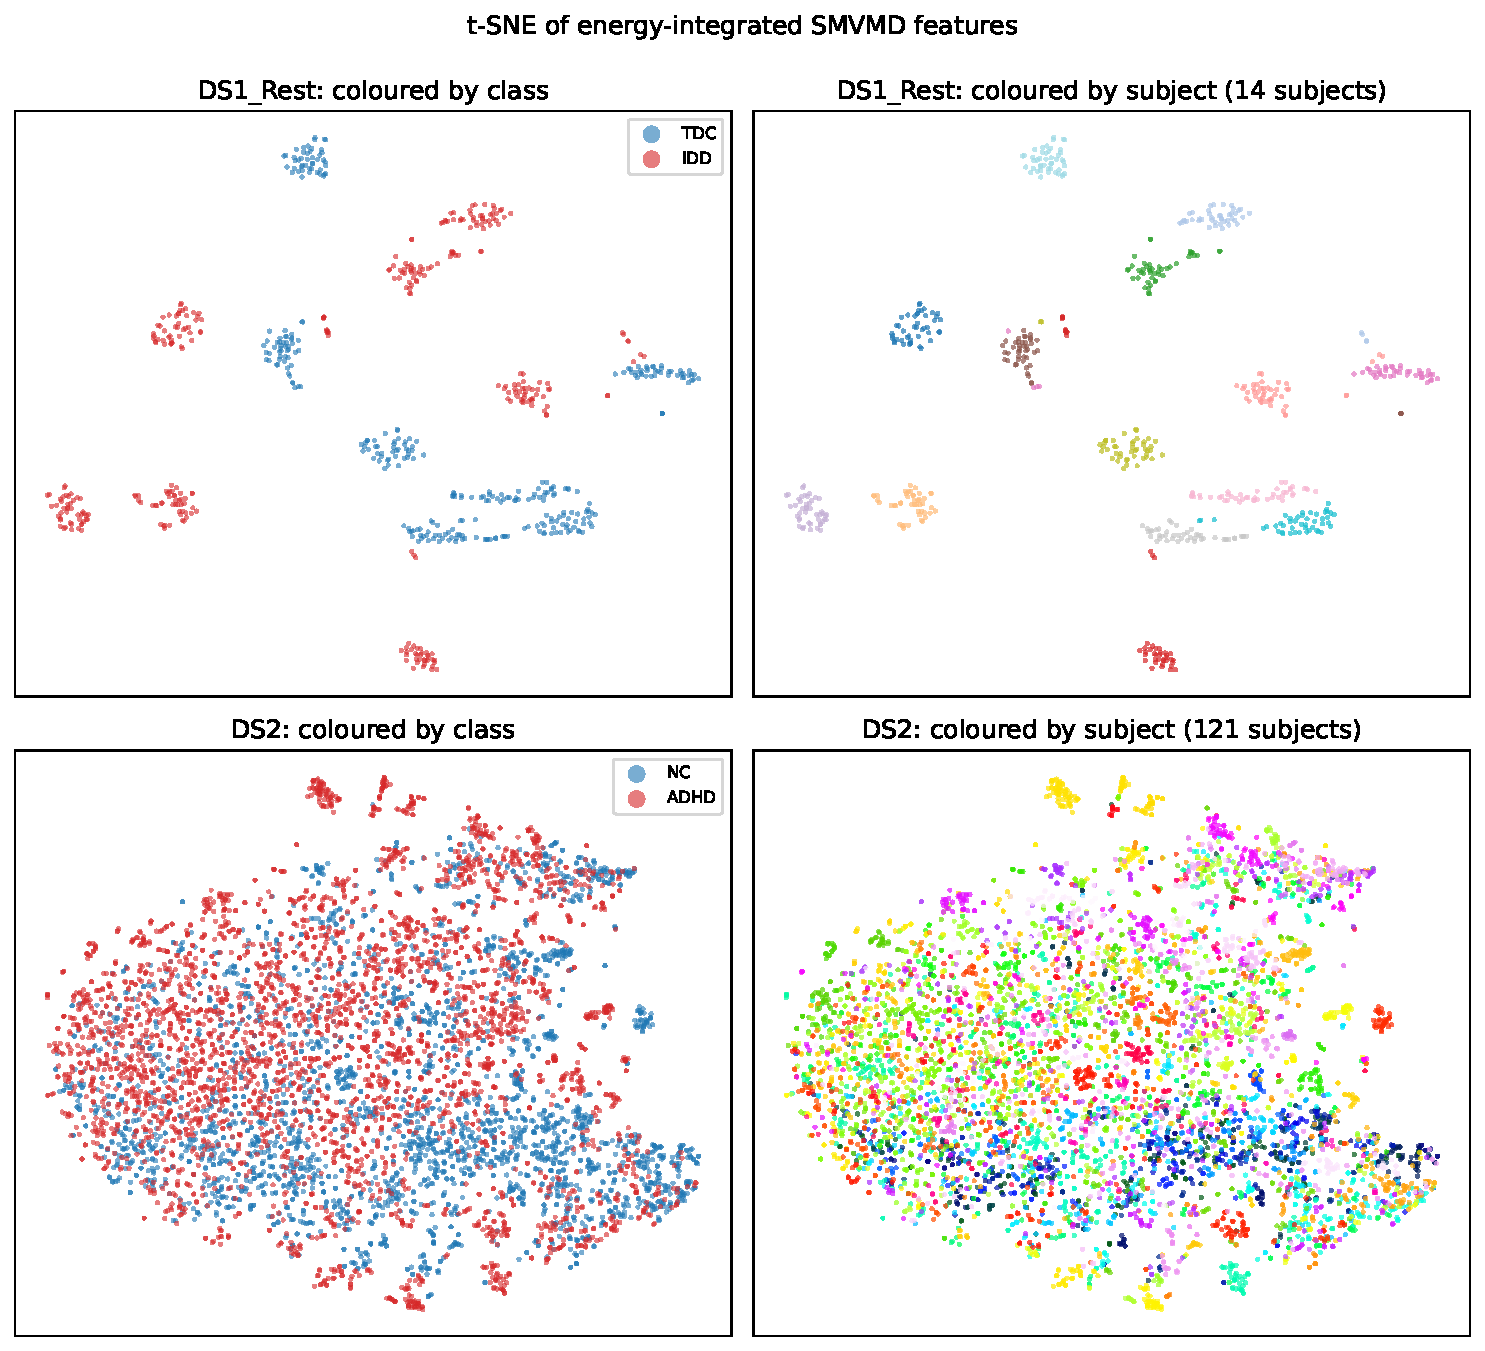
\includegraphics[width=0.66\textwidth]{figures/tsne_class_vs_subject.pdf}
\caption{t-SNE of the standardised energy-integrated
SMVMD features. Left: coloured by class; right: coloured by child. Top: DS-1
rest; bottom: DS-2.}
\label{fig:tsne}
\end{figure}

\textbf{What the features encode.} Figure~\ref{fig:tsne} projects the feature
vectors with t-SNE. In DS-1 the windows form one tight cluster per child; the
classes appear separated only because every child belongs to a single class. Table~\ref{tab:embed} quantifies this
with silhouette scores computed on class labels and on
child identity, and with a probe that predicts \emph{which child} produced a
window using a 1-nearest-neighbour classifier under segment-wise 10-fold CV.
The child is identified with \subjIDRest{} accuracy in DS-1 rest (chance
\subjIDchanceRest{}) and \subjIDAdhd{} in DS-2 (chance \subjIDchanceAdhd{}).
In DS-2 the child silhouette is negative, so children do not form compact
global clusters, yet a window's nearest neighbour still usually comes from
the same child.

\begin{table}[t]
\centering\footnotesize
\caption{Class versus child structure in the SMVMD feature space.}
\label{tab:embed}
\begin{tabular}{lcccc}
\toprule
Setting & Silhouette (class) & Silhouette (subject) & Subject ID, 1-NN & Chance\\
\midrule
DS-1 Rest & 0.075 & 0.218 & 98.91\% & 7.14\% \\
DS-1 Music & 0.066 & 0.193 & 99.07\% & 7.14\% \\
DS-1 Rest+Music & 0.067 & 0.173 & 99.30\% & 7.14\% \\
DS-2 & 0.026 & -0.150 & 65.39\% & 0.83\% \\
\bottomrule
\end{tabular}

\end{table}

\textbf{Raw-channel baseline.} The same nine features computed directly
on each preprocessed channel, without SMVMD, and passed through the same
pipeline give the right-hand columns of Table~\ref{tab:protocols}.

\begin{figure}[t]
\centering
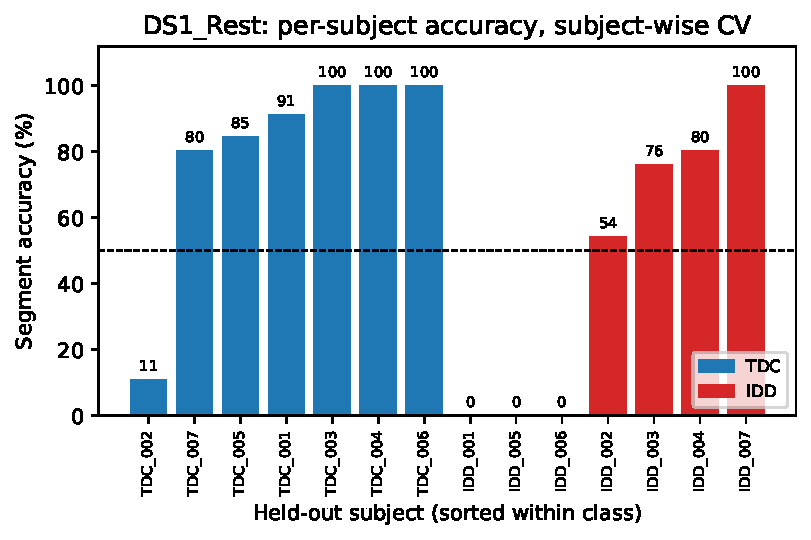
\includegraphics[width=0.49\textwidth]{figures/per_subject_accuracy_DS1_Rest.pdf}\hfill
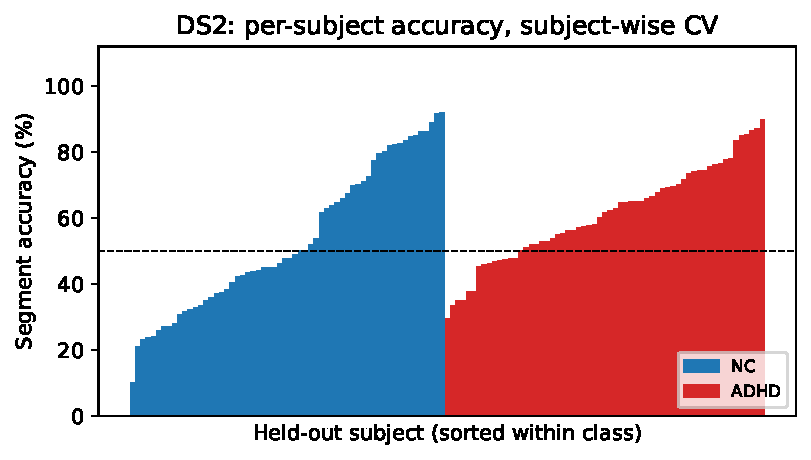
\includegraphics[width=0.49\textwidth]{figures/per_subject_accuracy_DS2.pdf}
\caption{Fraction of each held-out child's windows classified correctly under
subject-wise cross-validation. Left: DS-1 rest (LOSO); right: DS-2 (grouped
10-fold). The dashed line marks 50\%.}
\label{fig:persubj}
\end{figure}

\textbf{Per-child accuracy.} In DS-1 rest, errors fall on whole children
(Figure~\ref{fig:persubj}): \nPerfectRest{} children are correct in every
window and \nZeroRest{} are wrong in every window. In DS-2, per-child accuracy
varies continuously, and \nBelowHalfAdhd{} of \nSubjAdhd{} children have fewer
than half of their windows correct.

\begin{figure}[t]
\centering
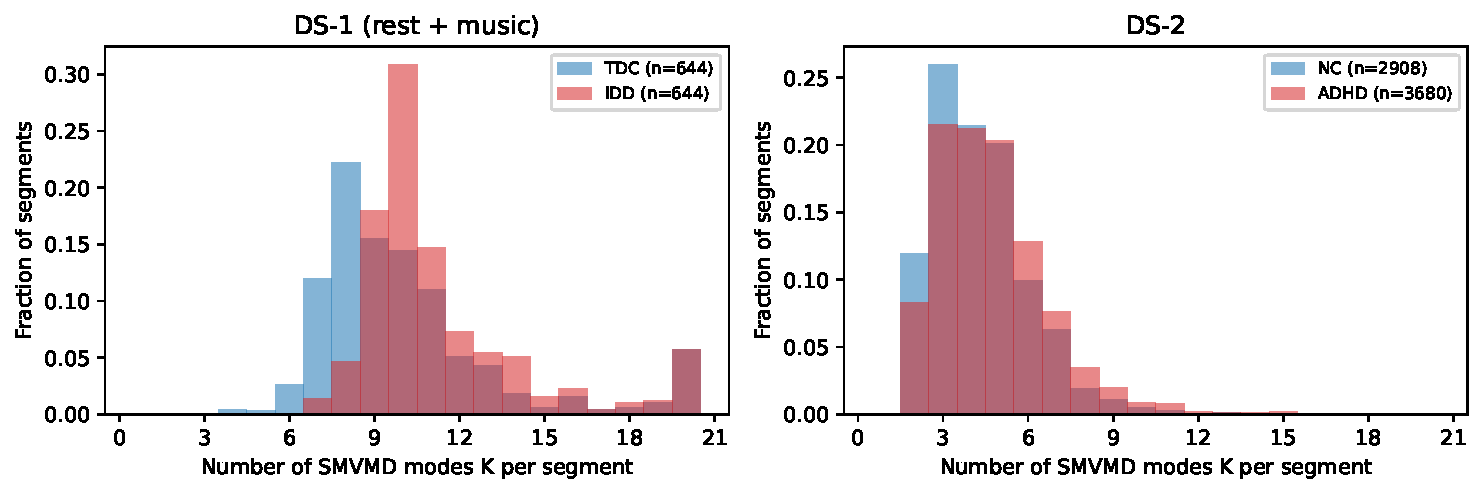
\includegraphics[width=0.86\textwidth]{figures/smvmd_mode_count_histogram.pdf}
\caption{Number of SMVMD modes per window, by dataset and class.}
\label{fig:modes}
\end{figure}

\textbf{Number of SMVMD modes.} Figure~\ref{fig:modes} shows the distribution
of $K$. DS-1 windows produce \modeMeanDsOne{} modes on average (IDD
\modeDisDsOne{}, TDC \modeCtlDsOne{}), and \modeCapDsOne{} of them stop at the
20-mode safety limit of the implementation. DS-2 windows produce
\modeMeanDsTwo{} (ADHD \modeDisDsTwo{}, NC \modeCtlDsTwo{}) and never reach the
limit.

\subsection{Discussion}

\textbf{Gap between protocols.} The analyses point to one explanation for
the large drop: the features describe each child far more distinctly than
they describe the diagnostic groups. A classifier that recognises a child from
that child's other windows inherits the child's label, which works only when
the child was seen in training. This is a property of the evaluation design
rather than of this particular pipeline, and segment-level splits are common
in the EEG literature (Table~\ref{tab:lit}). The subject-wise figures are the
relevant estimate for new children, although with \nSubjRest{} children each
DS-1 child accounts for \subjIDchanceRest{} of the windows, so these estimates
are coarse.

\textbf{Overlap and selection.} Removing overlap lowers DS-2 segment-wise
accuracy from \accSegFiftyAdhd{} to \accSegZeroAdhd{} but leaves its
subject-wise accuracy essentially unchanged (\accSubjFiftyAdhd{} to
\accSubjZeroAdhd{}), so samples shared between overlapping windows inflate the
segment-wise score; part of the drop may also come from halving the training
windows. On DS-1 the change is small, because the child signature is strong
enough without shared samples. Fitting mRMR on all data did not raise
accuracy, so selection leakage does not explain the segment-wise scores; the
effect of tuning hyperparameters on all data remains to be tested.

\textbf{Role of SMVMD.} Under subject-wise evaluation the raw-channel
features score higher than the SMVMD features on all three DS-1 settings and
are comparable on DS-2 (Table~\ref{tab:protocols}), even though the
hyperparameters were chosen in \cite{chandela2025} for SMVMD features. With
fixed hyperparameters, no benefit of the decomposition is visible yet; the
ablation study of Section~\ref{sec:plan} will test this properly. The number of
modes itself differs between classes, which suggests that $K$ carries
class-related information, but it may also be child-specific.

\textbf{Dataset confounds.} According to the DS-2 description, the children
with ADHD had been taking methylphenidate (Ritalin) for up to six months,
while controls were unmedicated \cite{motie2020,chandela2025}. Medication
status is thus perfectly aligned with the label, and a classifier cannot
distinguish ADHD from its treatment on this dataset. Recording length also
varies, so children contribute between \nSegPerSubjMinAdhd{} and
\nSegPerSubjMaxAdhd{} windows and are weighted unequally in segment-level
metrics; child-level reporting avoids this.

\textbf{Limitations of the current work.} Hyperparameters were taken from
\cite{chandela2025} rather than re-optimised; DS-1 uses the dataset's
preprocessed recordings instead of re-running independent component analysis;
and the SMVMD stopping rule, which \cite{chandela2025} does not specify, is
implemented as a residual-energy threshold with a 20-mode limit.

% =================================================================== 5
\section{Planned Workflow Timeline}
\label{sec:plan}

The project began in August 2026. Table~\ref{tab:plan} lists the work
completed up to the mid-semester evaluation on 25 September and the plan up to
the final evaluation and submission at the end of November. Every planned
experiment will keep all windows of a child on one side of the split and will
report child-level accuracy.

\begin{table}[h]
\centering\footnotesize
\caption{Project timeline (2026).}
\label{tab:plan}
\begin{tabularx}{\textwidth}{l X}
\toprule
Period & Work \\
\midrule
August -- 25 Sep & \emph{Completed:} study of the paper and datasets; Python
       reproduction of the full pipeline on DS-1 and DS-2; subject-wise
       evaluation, overlap, raw-channel and embedding analyses; this report.
       Mid-semester evaluation on 25 September. \\
28 Sep -- 11 Oct & Nested subject-wise cross-validation: Bayesian
       hyperparameter and feature-count search inside each outer fold;
       bootstrap confidence intervals over children. \\
12 -- 25 Oct & Ablation ladder under the nested protocol: raw channels
       $\rightarrow$ fixed frequency bands $\rightarrow$ VMD $\rightarrow$
       MVMD $\rightarrow$ SMVMD; sensitivity to the SMVMD stopping rule. \\
26 Oct -- 8 Nov & Interpretability: permutation importance and SHAP on
       subject-wise models, channel-level topographic maps, and a theta/beta
       power ratio baseline. \\
9 -- 15 Nov & Cross-dataset feature analysis on the 10 electrodes common to
       both datasets (F7, F3, F4, F8, T7, T8, P7, P8, O1, O2; T3/T4/T5/T6 in
       the DS-2 montage correspond to T7/T8/P7/P8). \\
16 -- 22 Nov & Channel reduction: performance of reduced electrode subsets
       under subject-wise evaluation. \\
23 -- 30 Nov & Consolidation and final report; final evaluation and
       submission at the end of November. \\
\bottomrule
\end{tabularx}
\end{table}

% =================================================================== 6
\footnotesize
\begin{thebibliography}{9}
\setlength{\itemsep}{0pt}

\bibitem{chandela2025} U. Chandela, K. N. Faisal, and R. R. Sharma,
``Electroencephalogram-based unified approach for multiple neurodevelopmental
disorders detection in children using successive multivariate variational mode
decomposition,'' \emph{IEEE Trans. Cogn. Develop. Syst.}, vol.~17, no.~6,
pp.~1350--1359, Dec. 2025.

\bibitem{sareen2020data} E. Sareen, L. Singh, B. Varkey, K. Achary, and
A. Gupta, ``EEG dataset of individuals with intellectual and developmental
disorder and healthy controls under rest and music stimuli,'' \emph{Data
Brief}, vol.~30, 2020, Art. no.~105488.

\bibitem{motie2020} A. Motie Nasrabadi, A. Allahverdy, M. Samavati, and
M. R. Mohammadi, ``EEG data for ADHD/control children,'' IEEE DataPort, 2020,
doi: 10.21227/rzfh-zn36.

\end{thebibliography}

\end{document}
